% =====================================================================
% Draft 4 SKELETON: "The Evidence Corpus"
% A Public Resource of Human-Curated Privacy-Policy Evidence Pointers
% and the Linguistics of Why Auditors Doubt.
% Target: International Journal of Human-Computer Studies.
% =====================================================================
\documentclass[11pt,a4paper]{article}

\usepackage[utf8]{inputenc}
\usepackage[T1]{fontenc}
\usepackage{lmodern}
\usepackage{microtype}
\usepackage[margin=2.4cm]{geometry}
\usepackage{graphicx}
\usepackage{xcolor}
\usepackage{booktabs}
\usepackage{array}
\usepackage{caption}
\usepackage{enumitem}
\usepackage{tikz}
\usepackage{pgfplots}
\usepackage{amsmath,amssymb}
\usepackage{url}
\usepackage[hidelinks]{hyperref}
\usepackage[round]{natbib}
\bibliographystyle{plainnat}

\pgfplotsset{compat=1.18}
\usetikzlibrary{arrows.meta,positioning,shapes.geometric,fit,calc,
                patterns,backgrounds,shadows}

\definecolor{dgBlue}   {RGB}{ 39, 99,178}
\definecolor{dgBlueL}  {RGB}{218,232,248}
\definecolor{dgOrange} {RGB}{226,123, 32}
\definecolor{dgOrangeL}{RGB}{252,229,205}
\definecolor{dgGreen}  {RGB}{ 84,156, 84}
\definecolor{dgGreenL} {RGB}{225,243,217}
\definecolor{dgPurple} {RGB}{132, 76,162}
\definecolor{dgPurpleL}{RGB}{233,221,242}
\definecolor{dgRed}    {RGB}{200, 64, 64}
\definecolor{dgRedL}   {RGB}{248,215,218}
\definecolor{dgTeal}   {RGB}{ 38,140,140}
\definecolor{dgTealL}  {RGB}{211,236,236}
\definecolor{dgGold}   {RGB}{218,165, 32}
\definecolor{dgGoldL}  {RGB}{251,236,196}
\definecolor{dgGrey}   {RGB}{ 90, 90, 90}
\definecolor{dgGreyL}  {RGB}{235,235,235}

\newcommand{\dataguard}{\textsc{DataGuard}}
\newcommand{\dec}[1]{\textsf{#1}}

\title{\bfseries The Evidence Corpus: \\
A Public Resource of Human-Curated \\
Privacy-Policy Evidence Pointers}
\author{Anonymous Author(s)\\\small (Skeleton draft for IJHCS submission)}
\date{}

\begin{document}
\maketitle

\begin{abstract}
\noindent\textbf{Skeleton draft.}
When a trained reviewer flags an Android Data Safety label as
\emph{Incorrect}, what part of the privacy policy do they point at?
We release the \dataguard{} Evidence Corpus: $4{,}623$ sentence-level
evidence excerpts paired with the structured Data Safety claim under
review, a four-way audit verdict, a free-text rationale, and annotator
metadata. We analyse linguistic features of the cited excerpts and find
that hedging language is over-represented in evidence cited for
\emph{Incorrect} verdicts ($28.0\%$ vs $21.7\%$), no-data language is
\emph{under}-represented ($9.4\%$ vs $14.6\%$), and third-party language
is verdict-neutral ($53$--$55\%$). We pair the corpus with a baseline
linguistic-feature classifier and translate the findings into three UI
affordances for evidence-grounded privacy review.
\end{abstract}

\noindent\textbf{Keywords:}\ privacy-policy corpus; evidence pointers;
audit linguistics; usable privacy; HCI dataset release.

\bigskip\hrule\bigskip

% =====================================================================
\section{Introduction}
% =====================================================================
A modern Android app exposes data practices through a short structured
Data Safety label~\citep{googledatasafety2022} and a long-form privacy
policy. When a reviewer judges that the label is inconsistent with the
policy, they do so by locating a fragment of the policy text. Until now
there has been \emph{no public resource} that captures these
fragment-level evidence pointers paired with the audit verdict.

\paragraph{What we release.} The \dataguard{} Evidence Corpus:
$4{,}623$ excerpts (median length $\sim 160$ chars, i.e.\ a sentence)
from $1{,}506$ judgments over $1{,}214$ Android apps in $12$ Google Play
categories, produced by seven trained annotators. Each excerpt is
linked to (i) the structured Data Safety claim under review,
(ii) a verdict on one of four axes (sharing-correct,
sharing-complete, collection-correct, collection-complete),
(iii) the annotator's free-text rationale, and (iv) annotator metadata.

\paragraph{What the corpus tells us.}
Hedging language and no-data language are diagnostic of audit verdicts;
third-party language is not. Both directions matter: hedging suggests
the auditor doubts the label, no-data language suggests the auditor
supports the label.

% =====================================================================
\section{Related work}
% =====================================================================
\paragraph{Privacy-policy corpora.}
OPP-115~\citep{wilson2016creation} provides $115$ policies with
fine-grained data-practice annotations. Subsequent work covers choice
provisions~\citep{sathyendra2017identifying} and vagueness
theory~\citep{bhatia2016theory}. None pair excerpts with downstream
audit verdicts.

\paragraph{Automated mismatch and labels.}
\citet{harkous2018polisis,andow2019policylint,andow2020policheck,zimmeck2019maps}
extract policy claims for compliance checks. For platform labels,
\citet{xiao2023lalaine} measure iOS labels and
\citet{khandelwal2024unpacking} the Google Data Safety section. Our
corpus complements these by providing reviewer-side evidence.

\paragraph{Evidence-grounded review.}
CLAUDETTE~\citep{lippi2019claudette} flags unfair ToS clauses by
returning evidence sentences. The DataGuard corpus does the same for
mobile privacy and adds the audit verdict.

% =====================================================================
\section{The DataGuard Evidence Corpus}
% =====================================================================
\subsection{Schema}
Each audit row contains four \texttt{relevant\_*} fields, one per
judgment axis. Figure~\ref{fig:schema} shows the link structure.

\begin{figure*}[t]
\centering
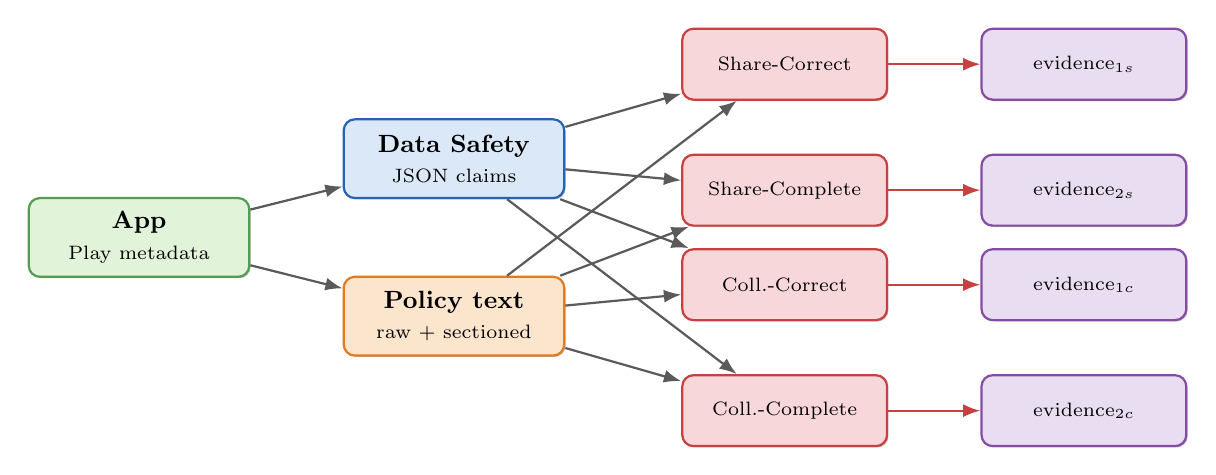
\begin{tikzpicture}[
  every node/.style={font=\small},
  >={Latex[length=2.2mm]},
  app/.style ={draw=dgGreen,fill=dgGreenL,thick,rounded corners=4pt,
               minimum width=2.8cm,minimum height=1.0cm,align=center,
               drop shadow={shadow xshift=0.5pt,shadow yshift=-0.5pt}},
  ds/.style ={draw=dgBlue,fill=dgBlueL,thick,rounded corners=4pt,
               minimum width=2.8cm,minimum height=1.0cm,align=center,
               drop shadow={shadow xshift=0.5pt,shadow yshift=-0.5pt}},
  pp/.style ={draw=dgOrange,fill=dgOrangeL,thick,rounded corners=4pt,
               minimum width=2.8cm,minimum height=1.0cm,align=center,
               drop shadow={shadow xshift=0.5pt,shadow yshift=-0.5pt}},
  ev/.style ={draw=dgPurple,fill=dgPurpleL,thick,rounded corners=4pt,
               minimum width=2.6cm,minimum height=0.9cm,align=center,
               font=\scriptsize,
               drop shadow={shadow xshift=0.5pt,shadow yshift=-0.5pt}},
  jud/.style={draw=dgRed,fill=dgRedL,thick,rounded corners=4pt,
               minimum width=2.6cm,minimum height=0.9cm,align=center,
               font=\scriptsize,
               drop shadow={shadow xshift=0.5pt,shadow yshift=-0.5pt}}
]
\node[app] (A) at (0,0) {\textbf{App}\\\scriptsize Play metadata};
\node[ds]  (DS) at (4,1) {\textbf{Data Safety}\\\scriptsize JSON claims};
\node[pp]  (PP) at (4,-1) {\textbf{Policy text}\\\scriptsize raw + sectioned};
\node[jud] (J1) at (8.2, 2.2) {Share-Correct};
\node[jud] (J2) at (8.2, 0.6) {Share-Complete};
\node[jud] (J3) at (8.2,-0.6) {Coll.-Correct};
\node[jud] (J4) at (8.2,-2.2) {Coll.-Complete};
\node[ev]  (E1) at (12.0, 2.2) {evidence$_{1s}$};
\node[ev]  (E2) at (12.0, 0.6) {evidence$_{2s}$};
\node[ev]  (E3) at (12.0,-0.6) {evidence$_{1c}$};
\node[ev]  (E4) at (12.0,-2.2) {evidence$_{2c}$};

\draw[->,thick,dgGrey] (A) -- (DS);
\draw[->,thick,dgGrey] (A) -- (PP);
\foreach \j in {J1,J2,J3,J4} \draw[->,thick,dgGrey] (DS) -- (\j);
\foreach \j in {J1,J2,J3,J4} \draw[->,thick,dgGrey] (PP) -- (\j);
\draw[->,thick,dgRed] (J1) -- (E1);
\draw[->,thick,dgRed] (J2) -- (E2);
\draw[->,thick,dgRed] (J3) -- (E3);
\draw[->,thick,dgRed] (J4) -- (E4);
\end{tikzpicture}
\caption{Evidence Corpus schema. Each audit row produces up to four
sentence-level evidence pointers, each paired with the structured
Data Safety claim it relates to.}
\label{fig:schema}
\end{figure*}

\subsection{Summary statistics}
Table~\ref{tab:corpus} reports per-field excerpt counts and length
distributions.

\begin{table}[t]
\centering\small
\caption{Per-field summary of the Evidence Corpus.}
\label{tab:corpus}
\begin{tabular}{lrrr}
\toprule
Field & Excerpts & Mean (chars) & Median \\
\midrule
relevant\_one\_s (share, correctness)  & 1{,}151 & 192 & 146 \\
relevant\_two\_s (share, completeness) & 1{,}021 & 215 & 173 \\
relevant\_one\_c (collect, correctness)  & 1{,}273 & 215 & 160 \\
relevant\_two\_c (collect, completeness) & 1{,}178 & 238 & 186 \\
\midrule
\textbf{Total}                          & \textbf{4{,}623} & --- & --- \\
\bottomrule
\end{tabular}
\end{table}

% =====================================================================
\section{Linguistic feature distribution}
% =====================================================================
We score each excerpt for four feature families:
\textbf{Hedging} (\emph{may, such as, including but not limited to,
reserve the right}),
\textbf{Third-party} (\emph{third-party, partner, vendor, service
provider, advertising, analytic, SDK, Google, Facebook}),
\textbf{Device IDs} (\emph{advertising ID, IP, cookie, MAC, Android ID,
identifier}),
and \textbf{No-data claims}
(\emph{do not collect, does not share, no personal, no data}).

\subsection{Verdict-discriminative distribution}
Restricting to evidence pasted under the \texttt{share-correct} judgment
and partitioning by verdict, we obtain Table~\ref{tab:disc}.

\begin{table}[t]
\centering\small
\caption{Marker prevalence in evidence cited under sharing-correctness.}
\label{tab:disc}
\begin{tabular}{lrrr}
\toprule
Marker family & Correct ($n=622$) & Incorrect ($n=511$) & $\Delta$ pp \\
\midrule
Hedging       & 21.7\% & \textbf{28.0\%} & $+6.3$ \\
Third-party   & 53.1\% & 55.4\% & $+2.3$ (neutral) \\
Device IDs    &  6.9\% &  8.0\% & $+1.1$ \\
No-data claim & \textbf{14.6\%} &  9.4\% & $-5.2$ \\
\bottomrule
\end{tabular}
\end{table}

% --- Figure: discriminative bars
\begin{figure}[t]
\centering
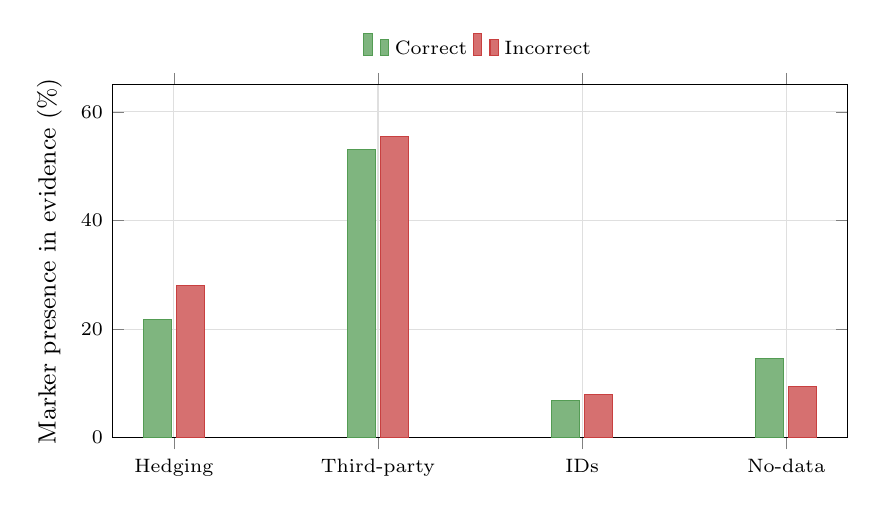
\begin{tikzpicture}
\begin{axis}[
  width=0.9\columnwidth,height=0.5\columnwidth,
  ybar,bar width=10pt,ymin=0,ymax=65,
  ylabel={Marker presence in evidence (\%)},
  symbolic x coords={Hedge,Third,IDs,NoData},
  xtick=data,
  xticklabels={Hedging,Third-party,IDs,No-data},
  x tick label style={font=\scriptsize},
  legend style={at={(0.5,1.04)},anchor=south,legend columns=2,
                draw=none,font=\scriptsize},
  grid=both,major grid style={draw=gray!25},minor grid style={draw=gray!10},
  tick label style={font=\scriptsize},label style={font=\small}
]
\addplot+[fill=dgGreen!75,draw=dgGreen] coordinates {
  (Hedge,21.7) (Third,53.1) (IDs,6.9) (NoData,14.6)};
\addplot+[fill=dgRed!75,draw=dgRed]     coordinates {
  (Hedge,28.0) (Third,55.4) (IDs,8.0) (NoData,9.4)};
\legend{Correct,Incorrect}
\end{axis}
\end{tikzpicture}
\caption{Linguistic-marker prevalence in evidence cited under
sharing-correctness, by verdict. Hedging and No-data are
discriminative; Third-party is verdict-neutral.}
\label{fig:disc}
\end{figure}

\subsection{Interpretation}
Two findings are counterintuitive.
(i) Third-party language is verdict-neutral: annotators cite "third party"
phrases when the label is Correct \emph{and} when it is Incorrect. The
mere mention of a third party does not predict a contradiction.
(ii) No-data language is \emph{more} prevalent in evidence cited as
Correct than Incorrect, meaning that policy text "we do not collect"
is used by annotators as evidence that the label is right.

% =====================================================================
\section{A baseline predictive model}
% =====================================================================
We frame share-correctness verdict prediction from the cited evidence
as binary classification with $4$ binary lexical features. A logistic
regression on the $n=1{,}133$ paired (evidence, verdict) rows reaches
$\sim 56$--$60\%$ accuracy --- above the $54.9\%$ majority baseline and
well below an LLM-based system; we report it as a transparent
floor that future LLM evidence-locators must beat to demonstrate value.

% =====================================================================
\section{Design implications}
% =====================================================================
\paragraph{A1 Hedging highlighter.} The audit UI should outline policy
text containing modal verbs and open-ended hedges. These spans were the
most diagnostic of audit doubt in our corpus.
\paragraph{A2 No-data confirmation prompt.} When the policy contains
explicit "we do not collect" language and the Data Safety section
declares no data, the UI should prompt the auditor to verify the
boundary of "personal" data rather than accept the label by default.
\paragraph{A3 Third-party recipient panel.} Because third-party
language is verdict-neutral on its own, the UI should not flag SDK
mentions automatically; it should let the auditor expand a recipient
panel to inspect each named third party.

% =====================================================================
\section{Limitations, release plan and conclusion}
% =====================================================================
\paragraph{Limitations.} Linguistic features are lexical, not semantic;
the corpus over-represents two annotators (acc 5 and 6 produced
$\sim 76\%$ of evidence excerpts); excerpts are sentence-grained but
not syntactically parsed.
\paragraph{Release plan.} We release the corpus as a CSV with the four
\texttt{relevant\_*} columns joined to per-judgment metadata
(annotator ID, app ID, verdict, rationale).
\paragraph{Conclusion.}
The Evidence Corpus is the first public resource that pairs
sentence-level policy excerpts with audit verdicts. It surfaces
verdict-discriminative linguistic features and grounds three concrete
UI affordances for evidence-grounded privacy review.

\bibliography{../draft-01-auditability-gap/references}

\end{document}
